%---------------------------------------------------------------------------
% System use cases.
%
%---------------------------------------------------------------------------
\section{Use cases}
\label{sec:ch4_usecases}

In this section one may find a usability analysis. This analysis is divided into 3 areas covering subsequent functional blocks: resources, measurements and visualizations. For each block, a diagram in the UML notation with an additional description is provided. This approach is equal to the second level of detail in writing use cases, as proposed by A. Cockburn\cite{0201702258}. 

Because the system is not expected to work with sensitive information, there are no authorization mechanisms or access control management considered in this work. This also implies that in all diagrams, there is only one actor: User.

\subsection{Resources Management}
\label{subsec:resources_mgmnt}

Figure \ref{fig:usecase_resources} shows a diagram depicting use cases related to resources management. This includes the most generic actions like adding a resource, removing a resource or viewing its state. Additionally the application enables the user to manage the life cycle of specific resources (e.g. threads, processes) - user can pause, stop or resume previously paused item. What should be also mentioned, this diagram covers indirect actions that might be performed by user, like selecting which internal monitor (the user might use more than one) should be used to manage a given resource, connecting to an external monitor, or even starting it.

\begin{figure}[ht]
\centering
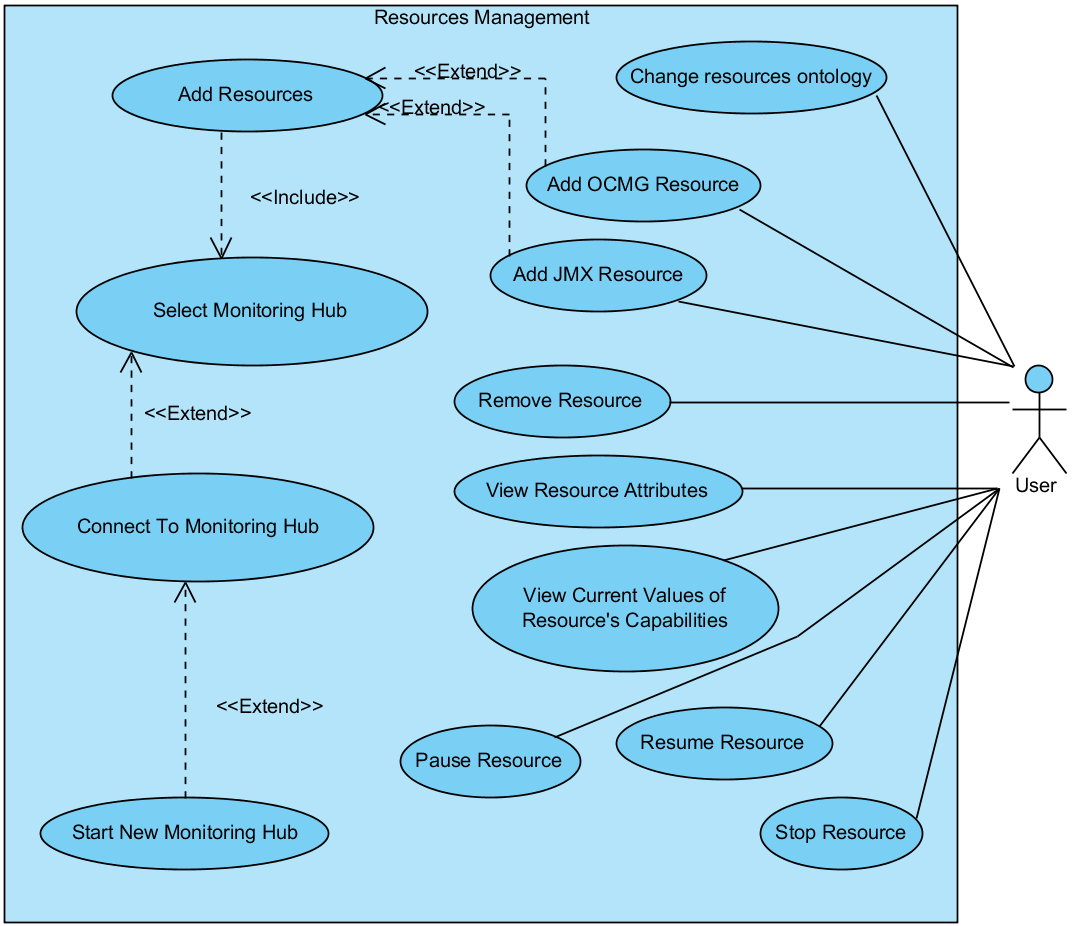
\includegraphics[width=0.8\textwidth]{resources}
\caption{Resources management use case diagram}
\label{fig:usecase_resources}
\end{figure}

The main use cases (actions performed by user directly to achieve his/hers aims) are as follows:

\begin{itemize}
\item {\bf Add an OCM-G Resource}~~~~~~~~~~~~~~~~~~~~~~~~~~~~~~~~~~~~~~~~~~~~~~~~~~~~~~~~\linebreak
Adding OCM-G resources. A OCM-G resource is a resource, monitored using the OCM-G monitoring system. This use case is a specialization of a more generic Add Resource use case. The user should be able to select application registered at the Main SM to monitor. After selecting an application, all its resources will be discovered and added to the resource tree.

\item {\bf Add a JMX Resource}~~~~~~~~~~~~~~~~~~~~~~~~~~~~~~~~~~~~~~~~~~~~~~~~~~~~~~~~\linebreak
Adding JMX resources. A JMX resource is a running JVM to which monitor can connect using the JMX protocol. While adding JMX resources, the user can arrange them into labeled clusters and applications, and must specify an URL that will be used by the monitoring component to connect to JVM.

\item {\bf Remove a Resource}~~~~~~~~~~~~~~~~~~~~~~~~~~~~~~~~~~~~~~~~~~~~~~~~~~~~~~~~\linebreak
Every added resource can be simply removed. All its measurements, and sub resources are removed as well.

\item {\bf View Resource Attributes} ~~~~~~~~~~~~~~~~~~~~~~~~~~~~~~~~~~~~~~~~~~~~~~~~~~~~~~~~\linebreak
By selecting a previously added resource, user should be able to view given resource's static attributes. This is highly specific to the resource type. For example, a process resource may have attributes like executable path, command line attributes, etc.

\item {\bf View Current Values of Resource's
Capabilities}~~~~~~~~~~~~~~~~~~~~~~~~~~~~~~~~~~~~~~~~~~~~~~~~~~~~~~~~\linebreak
After selecting a previously added resource, user can trigger fetching all resource\rq{}s capabilities values and thus view a snapshot of its state at a current moment of time.

\item {\bf Pause a Resource}~~~~~~~~~~~~~~~~~~~~~~~~~~~~~~~~~~~~~~~~~~~~~~~~~~~~~~~~\linebreak
User should be able to manage a resource\rq{}s life cycle, if applicable. Specific resources like threads, processes, or nodes can be paused, which freezes processing performed on a given resource.

\item {\bf Resume a Resource}~~~~~~~~~~~~~~~~~~~~~~~~~~~~~~~~~~~~~~~~~~~~~~~~~~~~~~~~\linebreak
As stated above, user can pause a resource. The user should be also able to resume a previously paused resource.

\item {\bf Stop a Resource}~~~~~~~~~~~~~~~~~~~~~~~~~~~~~~~~~~~~~~~~~~~~~~~~~~~~~~~~\linebreak
If a resource allows it, user should be able to stop the given resource totally. After stopping a resource, no further calculations can be performed using the given resource, and it is impossible to resume the resource again.

\item {\bf Change a Resources Ontology}~~~~~~~~~~~~~~~~~~~~~~~~~~~~~~~~~~~~~~~~~~~~~~~~~~~~~~~~\linebreak
The user can change the ontology that the system internally uses to build a resources tree. This change will not  be applied to the currently discovered resource tree, but all the newly added resources.

\end{itemize}


Indirect use cases (actions performed by user indirectly to help perform direct actions):

\begin{itemize}

\item {\bf Add a Resource}~~~~~~~~~~~~~~~~~~~~~~~~~~~~~~~~~~~~~~~~~~~~~~~~~~~~~~~~\linebreak
Generalization of use cases: Add JMX Resource and Add OCM-G Resource. It was extracted to ease the modeling of functionalities provided by those use cases, like selecting the monitoring component.

\item {\bf Select a Monitoring Hub}~~~~~~~~~~~~~~~~~~~~~~~~~~~~~~~~~~~~~~~~~~~~~~~~~~~~~~~~\linebreak
To be able to add a resource, the user has to select a monitor that will be responsible for managing resources and gathering data related to them.

\item {\bf Connect to a Monitoring component}~~~~~~~~~~~~~~~~~~~~~~~~~~~~~~~~~~~~~~~~~~~~~~~~~~~~~~~~\linebreak
User should be able, to connect to a manually started, potentially remote, monitor, prior to selecting one.

\item {\bf Start a new monitor}~~~~~~~~~~~~~~~~~~~~~~~~~~~~~~~~~~~~~~~~~~~~~~~~~~~~~~~~\linebreak
User should be able to start a new, potentially remote monitoring component, prior to connecting and using it.

\end{itemize}

\subsection{Measurements Management}
\label{subsec:measurement_mgmnt}



Figure~\ref{fig:usecases_measurements} shows the use cases related to the measurement management. Measurement functionalities are a bit less complex then the resources management. The user is able to create and start (which is merged into one action), stop, pause, resume measuring values of given capability. Additionally, the user can view all historical values, of a given measurement.

\begin{figure}[ht]
\centering
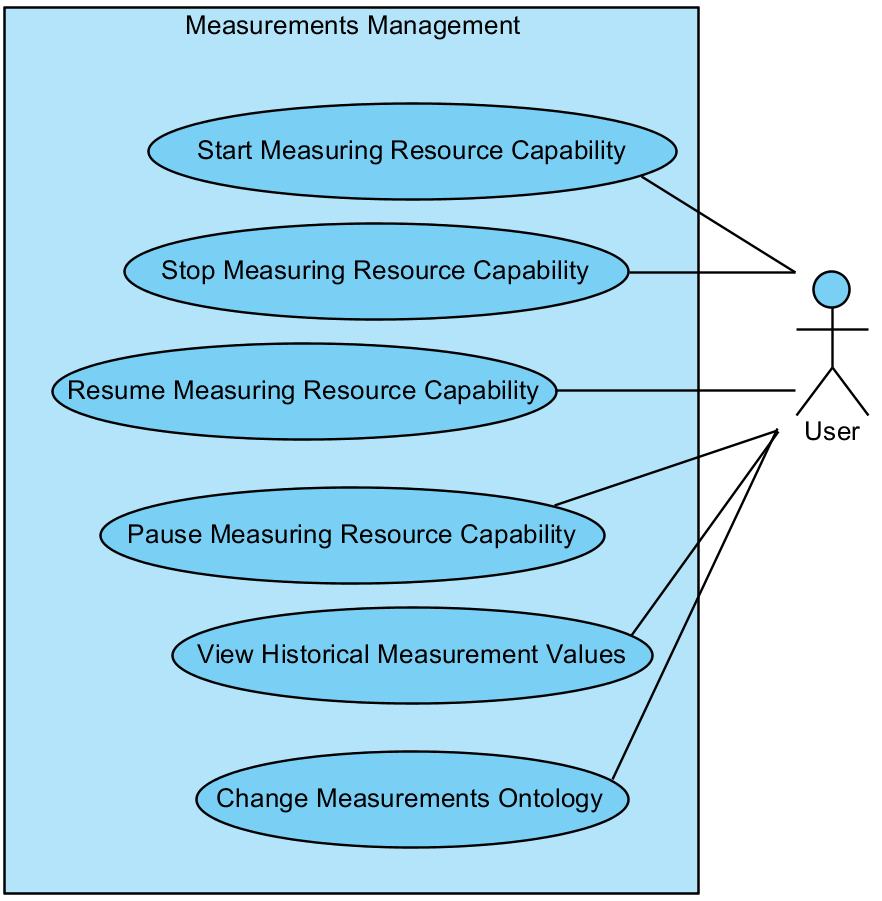
\includegraphics[width=0.5\textwidth]{Measurements}
\caption{Measurements management use case diagram}
\label{fig:usecases_measurements}
\end{figure}

\subsection{Visualizations Management}
\label{subsec:visualizations_mgmnt}

Figure~\ref{fig:usecases_visualisations} depicts the use cases related to the management of  measurement visualizations. The visualization functional block contains the following actions:

\begin{itemize}

\item {\bf Add a visualization}~~~~~~~~~~~~~~~~~~~~~~~~~~~~~~~~~~~~~~~~~~~~~~~~~~~~~~~~\linebreak
The user can add a new, empty (without any measurements attached) visualization. It is a basic first step that needs to be done to visualize measurements.

\item {\bf Add a measurement to a visualization}~~~~~~~~~~~~~~~~~~~~~~~~~~~~~~~~~~~~~~~~~~~~~~~~~~~~~~~~\linebreak
After creating a new visualization, the user can add a measurement, which makes the visualization component fully functional.

\item {\bf View a visualization}~~~~~~~~~~~~~~~~~~~~~~~~~~~~~~~~~~~~~~~~~~~~~~~~~~~~~~~~\linebreak
It is the most obvious use case - after creating a visualization and attaching a measurement, the user can view results of a measurement using the plots provided.

\item {\bf Remove a measurement from a visualization}~~~~~~~~~~~~~~~~~~~~~~~~~~~~~~~~~~~~~~~~~~~~~~~~~~~~~~~~\linebreak
The user should be able to remove a previously attached measurement from a given visualization.

\item {\bf Remove a visualization}~~~~~~~~~~~~~~~~~~~~~~~~~~~~~~~~~~~~~~~~~~~~~~~~~~~~~~~~\linebreak
When the user does not need a given visualization anymore, it can be simply removed.

\item {\bf Edit  visualization display options}~~~~~~~~~~~~~~~~~~~~~~~~~~~~~~~~~~~~~~~~~~~~~~~~~~~~~~~~\linebreak
The user should be able to have an additional level of control over a visualization. The management of a plot type makes it possible. The user should be able to change the display type of an already created visualization.

\item {\bf Change the measurements ontology}~~~~~~~~~~~~~~~~~~~~~~~~~~~~~~~~~~~~~~~~~~~~~~~~~~~~~~~~\linebreak
The user can change the ontology that defines the capabilities of a given resource.

\end{itemize}

\begin{figure}[ht]
\centering
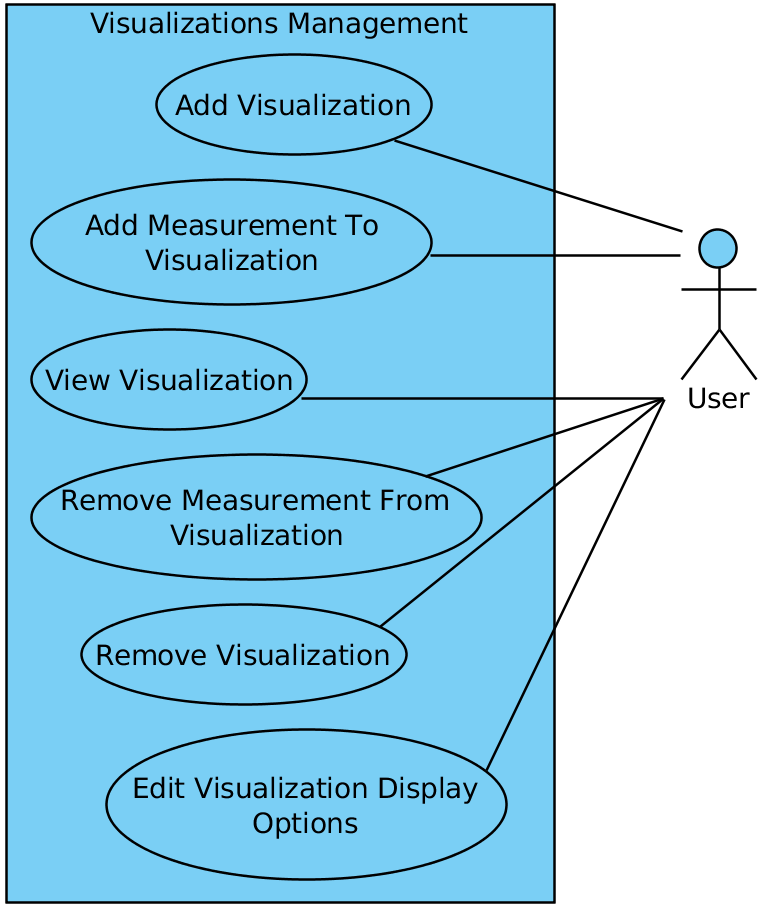
\includegraphics[width=0.4\textwidth]{Visualizations}
\caption{Use case diagram of visualizations management.}
\label{fig:usecases_visualisations}
\end{figure}
